\chapter{Project proposal} % (fold)
\label{cha:project_proposal}

In the Part \ref{part:overview_of_the_topic} we have presented the current state of the research of the P system variants. Especially the parallelism options have been investigated very well, but there are still some gaps that should be filled. For many variants the universality has been proven only when working in the maximally parallel mode. In most cases the sequential mode is strictly weaker, but this is not always true.

We have studied several variants of sequential P systems in order to obtain universality without using maximal parallelism.

\section{Sequential P systems without priorities with cooperative rules} % (fold)
\label{sec:sequential_p_systems_without_priorities_with_cooperative_rules}

A sequential variant without priorities and with cooperative rules is not univesal (see \cite{Ibarra04dang}). They have tried modifying the variant to make it universal and showed that with rules for membrane creation with unbounded number of membranes it became universal.

We tried other approach using rules with inhibitors. This variant is universal in both generating and accepting case and we don't even have to use membrane dissolution rules. In generative case the model is able to simulate maximal parallel P system and the accepting model can simulate a register machine.

Future plans include research other more restricted variants such as omitting cooperation in the rules or restrict the power of inhibitors.

\section{P systems with vacuum} % (fold)
\label{sec:p_systems_with_vacuum}

We propose a new variant of P system with vacuum in accordance with the criteria formulated in \cite{Besozzi:PhD:2004} (see beginning of the section \ref{sec:p_system_variants}). In the common sense, vacuum represents a state of space with no or a little matter in it. Using vacuum in modelling frameworks can help express certain phenomena more easily. We define a new P system variant, which creates a special vacuum object in a region as soon as the region becomes empty. The vacuum is removed whenever some object interacts with it. After the interaction, there is vacuum no longer. This removal process is realized by allowing the vacuum object to be used only on the left side of rules. If we made the vacuum to be removed automatically when an object enters the region, there would be no difference with the variant without vacuum objects because of no interactions with it.

We are interested in how the variant with the vacuum improves the computation power of a sequential P system in comparison to the variant without using the vacuum. This case have been shown to be universal.

In the future we will research other restriction for this variant such as non-cooperative rules, decaying objects, deterministic steps and will use techniques to show even non-universality results.

% section p_systems_with_vacuum (end)

% chapter project_proposal (end)

\chapter{Current status of the research} % (fold)
\label{cha:current_status_of_the_research}

\section{Sequential P systems without priorities with cooperative rules and inhibitors} % (fold)
\label{sec:sequential_p_systems_without_priorities_with_cooperative_rules_and_inhibitors}

Original definition of P systems with inhibitors (see \cite{Ionescu:jucs_10_5:on_p_systems_with}) allow to use only one inhibitor pre rule, e.g. $u\rightarrow v|_{\neg i}$. Alternative definition (see \cite{Agrigoroaiei:2010:Dissolution}) allow to use whole inhibitor set in the rule like $u\rightarrow v|_{\neg B}$, where $B$ is a set of objects. Such a rule can be applied only if no element of $B$ is present in the region.

For sequential P systems, the following lemma will show the equivalence of these definitions. However, special condition must be fulfilled, the regions with such rules cannot be empty.

% !TEX root = ../diz.tex
\begin{lemma}
\label{lemma:inhibitor_step}
  If there is at least one object present in each region of a P system, rewriting step in P system with inhibitor set can be simulated by multiple consecutive steps of P system with single inhibitor.
\end{lemma}

\begin{dokaz}
  Consider a P system with the alphabet $\Sigma$.
  For each rule $u\rightarrow v|_{\neg B}$, where $B=\{b_1, b_2, \dots ,b_n\}$ we will have rules:
    \begin{align*}
      c\rightarrow&c|GONE_{b}|_{\neg b} \text{~for all~} c\in \Sigma, b\in B \\
      u|GONE_{b_1}|GONE_{b_2}|\dots|GONE_{b_n}\rightarrow&v|GONE_{b_1}|GONE_{b_2}|\dots|GONE_{b_n}
    \end{align*}

\end{dokaz}

Note that symbols $GONE_b$ are created automatically when some object $c$ is present in the region. 

\begin{veta}
  The sequential P system with inhibitors defines the same Parikh image of language as P system with maximal parallelism.
\end{veta}

\begin{dokaz}
  We show that we can simulate maximal parallel step of P system with several steps of sequential P system with inhibitors. The proof is quite technical with some workarounds.

  % Membrane states

  It is important to note that in the maximal parallel step the rewriting occurs in all membranes, so we need to synchronize this process. Every membrane will have a state, represented as an object.

  The $RUN$ state represents that the rewriting still occurs. When there are no more rules to apply, the region has done its maximal parallel step and proceeds to the state $SYNCHRONIZE$. Other states are just technical - we need to implement sending objects between membranes and preparing for the next maximal parallel step by unmarking newly created objects in the current maximal parallel step, which have been marked to prevent double rewriting in one step.

  \begin{itemize}
    \item $RUN$: Rewriting occurs. Objects that are to be sent to the parent membrane are directly sent because the parent membrane is already in $RUN$ or $SYNCHRONIZE$ phase, so the $a^{\prime}$ symbols that are sent don't break anything. But objects that are to be sent down, cannot be sent immediately because child membranes can be in the previous phase waiting to restore symbols from previous step. Current symbols could interfere with them and be rewritten twice in this step. Such objects are only marked as ``to be sent down'': $a^{\downarrow\prime}$

    \item $SYNCHRONIZE$: Rewriting has ended and the membrane is waiting to get signal $SYNCED$ from the parent membrane to continue to the next step.

    \item $SENDDOWN$: Signal $SYNCED$ was caught and now all descendant membranes are in $SYNCHRONIZE$ phase so $a^{\downarrow\prime}$ can be sent down.

    \item $RESTORE$: All $a^{\prime}$ symbols are being restored to $a$, so the next step of rewriting can take place.
  \end{itemize}

  % Rewriting rules

  \begin{itemize}
    \item For every rule $r_i\in R$ such that
      \begin{align*}
        r_i = a_1^{M(a_1)}a_2^{M(a_2)}\dots a_n^{M(a_n)} \rightarrow a_1^{N(a_1)}a_2^{N(a_2)}\dots a_n^{N(a_n)}
      \end{align*}
      we will have the following rules:
      \begin{align*}
        &a_1^{M(a_1)-m_1}\dot{a}_1^{m_1}
        a_2^{M(a_2)-m_2}\dot{a}_2^{m_2}\dots
        a_n^{M(a_n)-m_n}\dot{a}_n^{m_n}|RUN \\
        \rightarrow &a_1^{\prime N(a_1)}a_2^{\prime N(a_2)}\dots a_n^{\prime N(a_n)}|RUN
      \end{align*}
      
      There will be such rule for each $0\leq m_i\leq M(a_i)$. It represents the idea that $\dot{a}$ can be used in rewriting in the same way as $a$. Right side of the rules contains symbols $a^\prime$, that prevents the symbols to be rewritten again.

    \item For every symbol $a\in V$ we will have the following rules:

    $a|RUN \rightarrow \dot{a}|RUN|_{\neg \dot{a}}$

    There will be at most one occurrence of $\dot{a}$.

    \item For every rule $r_i\in R$ there will be a rule that detects if the rule $r_i$ is not applicable. According to left side of the rule $r_i$, symbol $UNUSABLE_i$ will be created when there is not enough objects to fire the rule $r_i$. It means that left side of rule $r_i$ requires more instances of some object than are present in membrane.

    If the left side is of type:
    \begin{itemize}
      \item $a$: It is a context free rule. The rule can't be used if there is no occurrence of $a$ nor $\dot{a}$.

      $RUN \rightarrow UNUSABLE_i|RUN|_{\neg\{UNUSABLE_i, a, \dot{a}\}}$

      \item $ab$: It is a cooperative rule with two distinct objects on the left side. The rule cannot be used if there is one of them missing.

      $RUN \rightarrow UNUSABLE_i|RUN|_{\neg\{UNUSABLE_i, a, \dot{a}\}}$

      $RUN \rightarrow UNUSABLE_i|RUN|_{\neg\{UNUSABLE_i, b, \dot{b}\}}$

      \item $a^2$: It is a cooperative rule with two same objects. The rule can't be used if there is at most one occurrence of the symbol. That happens if there is no occurrence of $a$. There can still be $\dot{a}$, but at most one occurrence.

      $RUN \rightarrow UNUSABLE_i|RUN|_{\neg\{UNUSABLE_i, a\}}$
    \end{itemize}

    \item For every membrane with label $i$ there will be a rule:
    \begin{align*}
      &UNUSABLE_1|UNUSABLE_2|\dots|UNUSABLE_m|RUN \\
      \rightarrow &SYNCHRONIZE|SYNCTOKEN_i\uparrow
    \end{align*}

    If no rule can be used, maximal parallel step in the region is completed hence it goes to the synchronization phase and sends a synchronization token to the parent membrane.

    \item For every membrane there will be a rule:
    \begin{align*}
      &SYNCHRONIZE|SYNCTOKEN_j \\
      \rightarrow &SYNCHRONIZE|SYNCTOKEN_j\uparrow
    \end{align*}

    Membrane resends all synchronization tokens from child membranes to the parent membrane.

    \item In the skin membrane there is a rule which collects all the synchronization tokens from all membranes $1\dots k$ and then sends down signal that synchronization is complete. But before that, there can be some symbols that should be sent down, but they weren't, because the region below could have not started the rewriting phase that time. The result was just marked with $a^{\downarrow\prime}$.
    \begin{align*}
      &SYNCTOKEN_1|\dots|SYNCTOKEN_k|SYNCHRONIZE \\
      \rightarrow &SENDDOWN
    \end{align*}

    \item Every membrane other than skin membrane have to receive the signal to go to the senddown phase:

    $SYNCHRONIZE|SYNCED \rightarrow SENDDOWN$

    \item Every membrane will have rules for every symbol $a\in V$ to send down all unsent objects that should have been sent down:

    $SENDDOWN|a^{\downarrow\prime} \rightarrow SENDDOWN|a^{\prime}\downarrow$

    \item Every membrane will have a rule for detecting when all such objects have been sent and it goes to restore phase:

    $SENDDOWN \rightarrow RESTORE|_{\neg \{a_i^{\downarrow\prime}|1\leq i\leq n\}}$

    \item In the restore phase all symbols $a^{\prime}$ will be rewritten to $a$ in order to be able to be rewritten in the next maximal parallel step:

    $RESTORE|a^{\prime} \rightarrow RESTORE|a$
    
    \item When using lemma~\ref{lemma:inhibitor_step}, there may be some $GONE$ symbols left and now is the time to clear them:

    $RESTORE|GONE_i \rightarrow RESTORE$

    \item When the restore phase ends, it sends down a signal that all membranes have been already synchronized and next phase of rewriting has began in upper membranes:

    $RESTORE \rightarrow RUN|SYNCED\downarrow|_{\neg \{a_i^{\prime}|1\leq i\leq n\}\cup\{GONE_i|1\leq i\leq n\}}$
  \end{itemize}

  \definecolor{run}{rgb}{1,0.5,0}
  \definecolor{restore}{rgb}{0,0.5,0}
  \definecolor{synchronize}{rgb}{0,0,1}
  \definecolor{senddown}{rgb}{1,0,0}
  % Narrow texts in boxes
  \providecommand{\narrow}[1]{\scalebox{.85}[1.0]{#1}}

  \begin{figure}
    \def\svgwidth{\textwidth}
    \input{possible_pairs_of_states_of_parent_and_child_membrane.pdf_tex}
    % 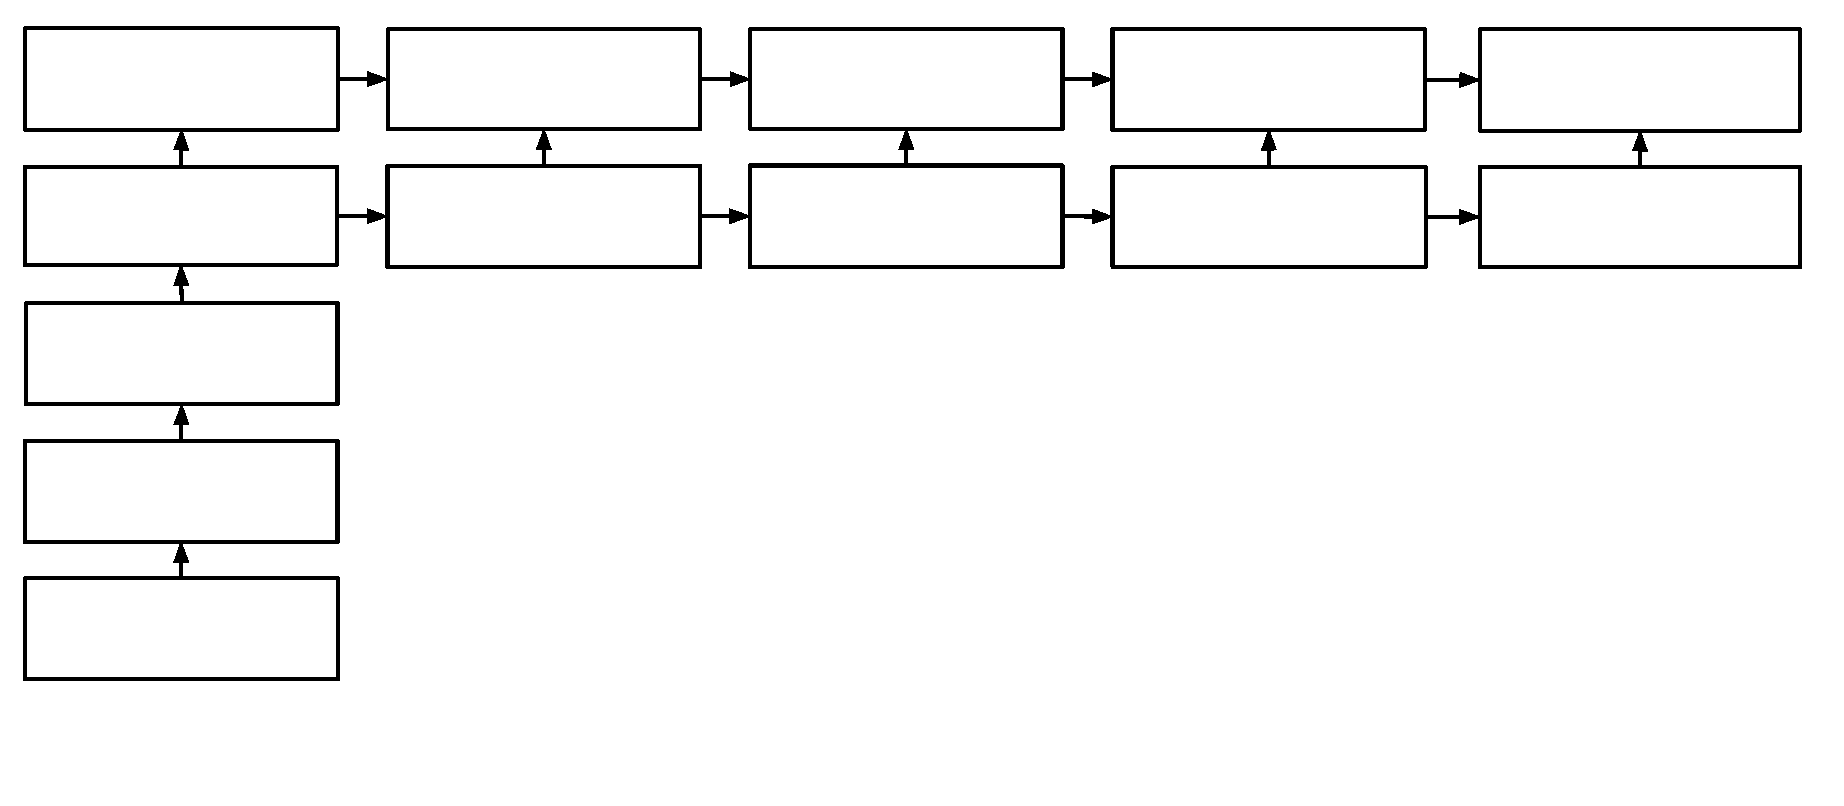
\includegraphics[width=\textwidth]{possible_pairs_of_states_of_parent_and_child_membrane}
    \caption{Possible pairs of states of parent and child membrane}
    \label{fig:possible_pairs_of_states_of_parent_and_child_membrane}
  \end{figure}

  \begin{figure}
    \def\svgwidth{\textwidth}
    \input{snapshot_of_all_membrane_states_while_simulating.pdf_tex}
    % 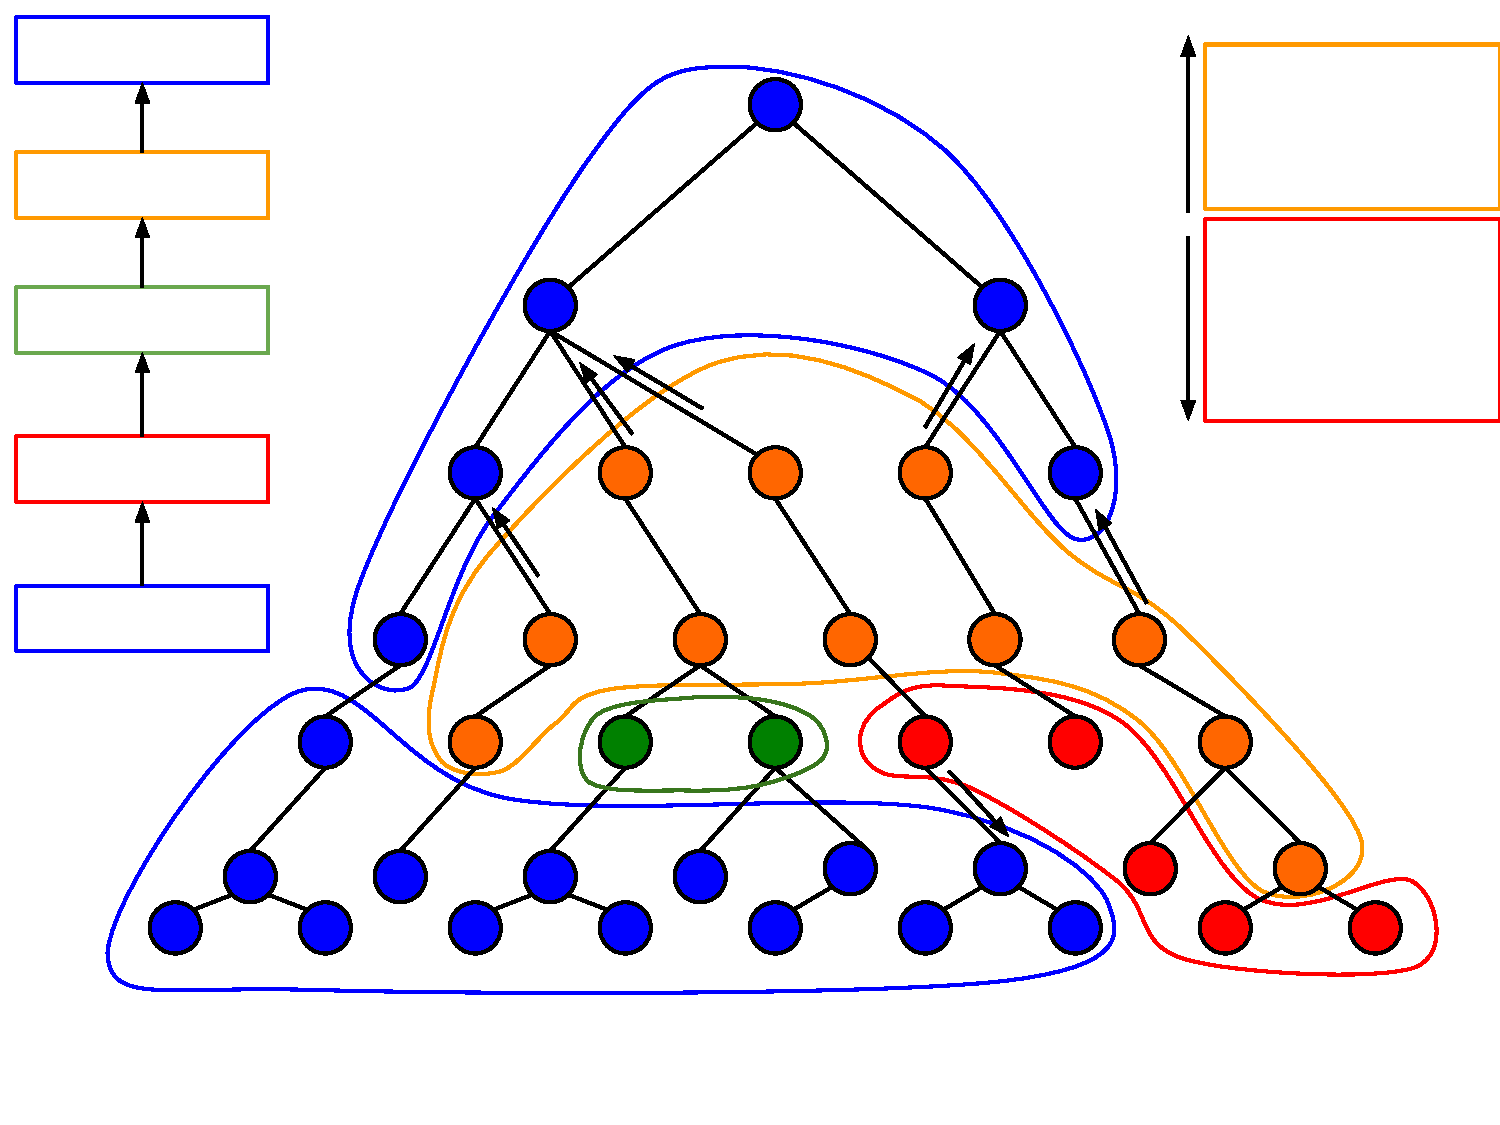
\includegraphics[width=\textwidth]{snapshot_of_all_membrane_states_while_simulating}
    \caption{Snapshot of all membrane states while simulating}
    \label{fig:snapshot_of_all_membrane_states_while_simulating}
  \end{figure}

  The pairs of possible phases of the parent and child membrane are shown in the figure \ref{fig:possible_pairs_of_states_of_parent_and_child_membrane} along with transitions between two consecutive global synchronizations - after the maximal parallel steps $i$ and $i+1$.

  In the figure \ref{fig:snapshot_of_all_membrane_states_while_simulating} the membrane structure is presented as a hierarchical structure. Every membrane is in one of four phases. It can be seen that the sending of the objects is performed in such phases that the receiving membrane is in either $RUN$ or $SYNCHRONIZE$ phase, so the received objects (marked $a^\prime$) does not interfere with rewriting.

  Another interesting idea can be seen in the figure \ref{fig:snapshot_of_all_membrane_states_while_simulating} that when a region is in the $SENDDOWN$ phase and objects are sent through the child membrane, the receiving region is in the $SYNCHRONIZE$ phase waiting for the $SYNCED$ signal, which will be sent to it when $SENDDOWN$ and $RESTORE$ phases finished.

  All membranes are nonempty during the simulation because at least the object representing the current phase is always present. By lemma~\ref{lemma:inhibitor_step} the rules with set of inhibitors can be simulated by single inhibitors.


\end{dokaz}




We have also reached this result in the accepting case by simulation of register machines.

\begin{veta}
  Sequential P systems with inhibitors can simulate register machines and thus equal $PsRE$.
\end{veta}


\begin{dokaz}
\label{proof:reg_by_inh}
  Suppose we have a $n$-register machine $M = (n,P,i,h)$. In our simulation we will have a membrane structure consisting of one membrane and the contents of register $j$ will be represented by the multiplicity of the object $a_j$.

  We will have P system $(V, \mu, w, R)$, where:
  \begin{itemize}
    \item $V$ is an alphabet consisting of symbols that represent registers $a_1,\dots a_n$ and instruction labels in $Lab(M)$,
    \item $\mu$ is a membrane structure consisting of only one membrane,
    \item $w$ is initial contents of the membrane. It contains symbols for the input for the machine $a_i^{n_i}$ where $n_i$ is initial state of register with label $i$ and initial instruction $e \in Lab(M)$.
    \item $R$ is the set of rules in the skin membrane:
    
    For all instructions of type $(e : add(j), f)$ we will have rule:
    \begin{itemize}
      \item $e \rightarrow a_j|f$.
    \end{itemize}
    
    For all instructions of type $(e : sub(j), f, z)$ we will have rules:
    \begin{itemize}
      \item $e|a_j \rightarrow f$ and
      \item $e \rightarrow z|_{\neg a_j}$.
    \end{itemize}

    And finally halting rules:
    \begin{itemize}
      \item $h|a_j \rightarrow h|\#$ for all $a\leq j\leq n$,
      \item $\# \rightarrow \#$,
    \end{itemize}
  \end{itemize}

  When the halting instruction is reached, if there is an object present in the membrane, the hash symbol $\#$ is created and it will cycle forever. If there is no object present, there is no rule to apply and computation will halt. It corresponds to the condition that all registers should be empty when halting.
\end{dokaz}

% section sequential_p_systems_without_priorities_with_cooperative_rules_and_inhibitors (end)

\section{Universality results of P systems with vacuum} % (fold)
\label{sec:universality_results_of_p_systems_with_vacuum}

\begin{veta}
  The sequential P system with Vacuum is universal.
\end{veta}

\begin{dokaz}
  We can simulate the variant of P system where the only cooperative rule is of type $a|a \rightarrow b$. According to \cite{Ibarra04dang} the variant, where the only cooperative rule is when both objects are the same, is universal. If there is no rule $a \rightarrow b$, we can rewrite $a$ to $a^{\prime}$ so we can mark all present symbols. $a^{\prime}$ symbols are kept in special membrane so the Vacuum can be created in main membrane and we can synchronize.
  
  But we won't do this madness again.
  
  Instead, we will try to prove universality by simulating the register machine. We need to detect when the current register is empty. If there was a symbol for every register as in the proof~\ref{proof:reg_by_inh}, the Vacuum would be created only if all registers are empty. But the $sub()$ instruction need to detect when one concrete register is empty.
  
  We will have a membrane for each register. That membrane will be contained in the skin membrane. The number of objects in membrane $i$ will correspond to the value of register $i$.
  
  The alphabet will consist of instruction labels and register counter $a$. The skin membrane will only have an instruction label. It is sent to corresponding membrane where the instruction is executed. Then, the following instruction is sent back to the skin membrane.
  
  We will have following rules in the skin membrane:
  
  \begin{itemize}
  \item $e \rightarrow e\downarrow_j$ for an instruction of type $e : add(j), f$ or $e : sub(j), f, z$ and
  \item $h \rightarrow h\downarrow$ for a halting instruction h.
  \end{itemize}
  
  And in non-skin membranes:
  
  \begin{itemize}
  \item $e \rightarrow a|f\uparrow$ instructions of type $e : add(j), f$,
  \item $e|a \rightarrow f\uparrow$ for instructions of type $e : sub(j), f, z$,
  \item $e|VACUUM \rightarrow z\uparrow$ for instructions of type $e : sub(j), f, z$, and
  \item $h|a \rightarrow h|a$
  \end{itemize}

  When halting, if there is an nonempty register, it will cycle forever with the last rule. However, if all registers are empty, the halting instruction label will stay in all membranes and the computation will halt.
  
\end{dokaz}

% section universality_results_of_p_systems_with_vacuum (end)

% chapter current_status_of_the_research (end)

